\documentclass[conference]{IEEEtran}
%\IEEEoverridecommandlockouts
% The preceding line is only needed to identify funding in the first
% footnote. If that is unneeded, please comment it out.
\usepackage[british]{babel}
\usepackage[noadjust]{cite}
\usepackage{url}
\usepackage[hyphenbreaks]{breakurl}
\usepackage{amsmath,amssymb,amsfonts}
\usepackage{algorithmic}
\usepackage{graphicx}
\usepackage{tabularx}
\usepackage[pdftex,colorlinks=true]{hyperref}
\def\UrlBreaks{\do\/\do-}

\begin{document}

\title{The Institute of Coding:\\A University-Industry Collaboration
  to\\Address the UK's Digital Skills Crisis}

% \author{\IEEEauthorblockN{James H. Davenport\IEEEauthorrefmark{1}, Tom
%     Crick\IEEEauthorrefmark{2}, Rachid Hourizi\IEEEauthorrefmark{1}}
% \IEEEauthorblockA{\IEEEauthorrefmark{1}Department of Computer Science, 
% University of Bath, Bath, UK\\
% Email: \{j.h.davenport,r.hourizi\}@bath.ac.uk} % \orcid{0000-0002-3982-7545}
% \IEEEauthorblockA{\IEEEauthorrefmark{2}School of Education, 
% Swansea University, Swansea, UK\\
% Email: thomas.crick@swansea.ac.uk}} % \orcid{0000-0001-5196-9389}
 
\maketitle

\begin{abstract}
The Institute of Coding is a new \pounds40m+ initiative by the UK
Government to ``transform the digital skills profile of the
country''. In the context of widespread national and international
educational and economic policy interventions, it responds to the
apparently contradictory data that the UK has a digital skills
shortage across a variety of sectors, yet its higher education system
produces computing graduates every year who end up unemployed, or
underemployed.

The Institute is a large-scale national intervention to address some
of the perceived issues with formal educational routes versus
industry-focused skills and training, for example: technical skills
versus ``soft'' or ``work-ready'' skills; industry-readiness versus
``deep education''; inclusion and diversity of the current and future
technical workforce; and managing expectations for the broad digital,
data and computational skills demands of employers across a wide range
of economic sectors.

All of this is taking place at the higher education/industry interface
at the same time as substantial computer science curriculum reform
across the four nations of the UK -- especially in England, with a new
statutory computing curriculum from 2014 (the first products of which
are just commencing their university education), in which all children
are expected to learn two programming languages, as well as wider
computer science fundamentals and develop transferable computational
thinking skills.

In this paper, we describe the background, evidence base and rationale
for the Institute of Coding (especially within the complex UK policy
context); its key themes, current activities and outputs; as well as
anticipate its likely impact over the coming years. Furthermore, we
reflect on the potential replicability of aspects of the Institute
(and related initiatives in the UK) to other nations or regions with
similar ambitions to address the ``digital skills crisis''.
\end{abstract}

\begin{IEEEkeywords}
Digital skills, Programming, Computer science education, Undergraduate
education, Graduate education, Industry collaboration
\end{IEEEkeywords}

\section{Introduction}

% TC: need more UK context here, I can add this -- do we want to have
% this framed as a paper to justify/introduce the IoC, as well as
% other UK interventions? Framed as a discussion piece with
% transferability elsewhere?
%Set the scene -- UK digital skills, CS ed reform, digital economy, etc

We are frequently being told that this is ``the digital age'', and
that we ``live in a knowledge economy''\footnote{Despite the debunking
by Friesen~\cite{Friesen2008}.}, with ``software eating the
world''~\cite{andreessen:2011}; nevertheless, the impact of digital on
all of our lives is clear. From entertainment and communication, via
the power and reach of an oligopoly of social media platforms, with
``algorithms'' influencing what news we consume, or making decisions
that affect us every day; to education, health and social care,
through to innovation in public services~\cite{ecdsmsuk:2018}. We are
also seeing the emergence of artificial intelligence and machine
learning as general-purpose technologies that could transform whole
industries and even re-invent the process of invention
itself~\cite{brynjolfsson-et-al:2018,dwivedi-et-al:ijim2019}. What
does this mean for education systems, national curricula and skills
training -- from compulsory, through to post-compulsory, into lifelong
learning?

\subsection{Defining the ``Digital Economy''}

Providing a comprehensive definition of the `digital economy' is
challenging; the OECD's 2002 definition of the ICT sector does not
provide much insight: ``{\emph{...a combination of manufacturing and
services industries that capture, transmit and display data and
information electronically}}''~\cite{oecd:2002}.  According to the
current -- but published in 2007! -- UK Standard Industrial
Classification of Economic Activities~\cite{onssic:2009}, the
``Information and Communication'' sector includes telecommunications,
computer programming, information services, as well as a wide range of
creative, publishing and broadcasting activities. Formal sector
classifications aside, it is clear that while the UK has had a
traditional vertical `IT and Telecoms' sector, it also increasingly
has a crucial enabling and facilitative horizontal digital sector. In
essence: there is no such thing as the `digital economy' -- our
economy is digital. While this situation is certainly not unique to
the UK, it is perhaps exemplified by some of the grand challenges
identified as part of the UK Industrial Strategy~\cite{ukis:2017},
published in 2017: from precision medicine, manufacturing and future
materials, to creative industries clusters and next generation
services, through to driverless cars and smart
cities~\cite{tryfonas+crick:petra2018}.

%\subsection{Diversity, especially Gender}\label{sec:Gender}

In 2018, the UK digital sector (as defined by OECD/UN Standard
Industry Classifications) comprised of 1.5 million jobs (4.5\% of the
total number of jobs in the UK), the highest number for the sector
(and a 16.1\% increase) since 2011~\cite{dcms:2018}. 49.7\% of these
are in ``{\emph{Computer programming, consultancy and related
activities}}'': precisely the area to which the Institute of Coding is
aimed. Its workers are more productive, on average, by \pounds10,000
per worker and jobs requiring digital tech skills command higher
salaries, at \pounds42,578 compared to \pounds32,477 for those that do
not. Despite the stereotype that digital tech jobs are for
``millennials'', 72\% of workers are aged over 35; however, only 19\%
of the UK digital tech workforce is
female~\cite{technation:2018}. Indeed, the Institute of Coding
announcement in 2018 quoted the even more pessimistic ``In 2017,
female programmers and software developers made up just 3.9 per cent
of tech and telco professionals in the UK''~\cite{DfE2018a}.

\subsection{Education and Skills Policy}

Globally, there are a plethora of high-profile initiatives and
interventions to address the wider societal challenge, and the
corresponding skills shortages, of our digital
world~\cite{cece:2017}. While there is a strong socio-economic focus,
it should not just be about jobs: we want, and need, a digitally
competent, capable and engaged citizenry. But this idealistic ambition
provides significant challenges for long-term, coherent, sustainable
policymaking and investment. More importantly, what do we mean by
digital skills? In recent years, we have seen a multitude of policy
reviews and reports from across government, academia, think tanks,
learned societies and charities that have attempted to encapsulate
some of the issues, as well as identifying potential solutions. At
least three recent UK Parliamentary Select Committee
inquiries~\cite{ukholds:2015,ukhocst:2016,ukholc:2017} have, wholly or
in part, focused on the `digital skills crisis'. They have all made a
number of specific recommendations, from curriculum and qualifications
reform, ensuring young people are safe online, improving professional
learning for practitioners, investment in infrastructure, developing
effective pedagogies and the wider educational research base in the
UK, through to terminology, fixing `leaky pipelines' and changing the
wider public perceptions of digital/technology disciplines.

Alongside substantial curriculum reform across the
UK~\cite{crick+sentance:2011,brown-et-al:sigcse2013,brown-et-al:toce2014},
including a new national curriculum in England~\cite{DfE2013a} and
emerging reform in
Wales~\cite{wgictreview:2013,crick+beauchamp:bera2017,moller+crick:jce2018},
we have also seen significant changes to the available qualifications,
based on perceived rigour, content, distinctiveness and modes of
assessment. The publication in 2017 by the Royal Society of a follow-up
to their 2012 report~\cite{rs:2012} on computing education in the
UK~\cite{rs:2017} framed some of these national challenges in the
context of computing for all, calling for a coherent strategy so that
all learners are equipped and empowered with the necessary skills to
be effective in the digital world.

However, it is clear that from all of these various reviews, reports,
activities, initiatives and interventions, there remains a lack of
policy coherency and connectedness -- more so when it cuts across
ministerial portfolios, or requires multi-year coordinated support. In
this paper we frame some of these strategic challenges -- and
opportunities -- and introduce the Institute of Coding, a new
\pounds40m+ initiative by the UK Government (but focused on England,
with related activity in Wales) to transform the digital skills
profile of the country~\cite{davenport-et-al:cep2019}.

The structure of the paper is as follows. In Section~\ref{problem} we
attempt to define the wider problem through the lens of graduate
employment and earnings; this is followed in Section~\ref{ukhepolicy}
by the UK higher education policy context and the skills mismatch
respectively; in Section~\ref{ioc} we present the Institute of Coding,
its key themes, activities and outputs, finishing with future work and the
potential replicability of aspects of the Institute in
Section~\ref{concl}.

% and now in Lithuania \cite{Xinhua2018a}) to prisons \cite{Maher2018a}.

\subsection{A Note on Nomenclature}

While in many instances throughout this paper we will refer to the
United Kingdom (UK) -- consisting of the four nations of England,
Scotland, Wales and Northern Ireland -- many of the initiatives,
approaches and funding models are specifically focused on England (or
England and Wales), as a number of policy areas, including education
and skills, are devolved to the respective national governments. We will
attempt to be as clear as possible when referring to specific
interventions across or between the four nations.

\section{So What's the Problem?}\label{problem}

Superficially, the employment outlook for computing graduates in the
UK looks excellent. A 2015 report from the UK Commission for
Employment and Skills~\cite[p.~74]{UKCES2015b} states:

\begin{quote} ...``{\emph{the digital sub-sector will need 518,000 workers for
roles in the three highest skilled occupational groups. However, over
the last ten years only 164,000 individuals graduated from a first
degree in computer science.}}''
\end{quote} 

This is beneficial to the individual: according to a 2011 UK
Government report on economic returns from higher education
qualifications~\cite[Figure 4]{BIS2011a}, ``mathematical and
computer sciences'' have the second highest earnings return of all
subjects (overtaken only by ``medicine and dentistry'').  The country
profits from this as well: per head, it is the fourth most beneficial
subject to the UK~\cite[p.~16]{BIS2011a}. Nevertheless, despite the
headline success in a variety of UK Government reports, the employment
figures are not good, and the earnings data are patchy.

\subsection{Graduate Employment}

Further to the 2015 UK education and skills report~\cite{UKCES2015b},
the following was highlighted in the 2016 UK Government
review of computer sciences degree accreditation and graduate
employability~\cite{Shadbolt2016a}, led by Sir Nigel Shadbolt:

\begin{quote} ``{\emph{In this context, apparently high rates of
unemployment\footnote{11.7\% six months after graduation (the then standard
UK measure) at the time of \cite{Shadbolt2016a}, compared with a STEM
average of 8.4\%. Note, however, that Computing is 20\% of STEM
\cite[Table 1]{Wakeham2016a}, so `STEM-less-Computing' has a 7.6\%
unemployment rate.} amongst graduates of Computer Sciences and other
STEM\footnote{STEM is ``Science, Technology, Engineering,
Mathematics'' for \cite{Shadbolt2016a} and this paper.} courses
demanded an explanation.}}
\end{quote}

A significant explanation is ``{\emph{There are notable differences in the
characteristics of Computer Sciences entrants compared to entrants in
other STEM subjects}}''~\cite[\P2.6]{Shadbolt2016a}: fewer women, but:

\begin{description}
\item[50\% ]more mature students;
\item[16\% ]more Black and Minority Ethnic (BME); and
\item[40\% ]more students from backgrounds where people have
traditionally not participated in HE (LPNs: low participation
neighbourhoods).
\end{description}

UK Government data suggests that Mature, BME and LPN students all find
getting jobs more difficult. However, for those students that do find
jobs, the data are better, showing fewer students in ``non-graduate
jobs'' or low-earning jobs than in STEM as a whole~\cite[Figure
6]{Shadbolt2016a}.

\subsection{Graduate Earnings}
If we look beyond purely getting jobs to the earnings\footnote{Clearly
not the only measure of job quality, or contribution to society, but
at least it is measurable, and has been measured in the UK graduate
longitudinal education outcomes (LEO) dataset~\cite{DfE2017a}, which
tracks individuals through school, university and into the labour
market, combining educational, tax and benefits data.}, the position
(as described in official government figures~\cite{DfE2018d}, and
analysed by the national media~\cite{BBC2018f}, which also allows the
reader to break down the data by university and subject) is even less
clear at a micro level, though at a macro level it
supports the 2016 Shadbolt review findings~\cite{Shadbolt2016a}.

At the macro level, we consider UK labour market returns~\cite[Table
5]{DfE2018d}. We focus on the `Men' data as presented here, as there
are (regrettably) many more than there are women in the cohorts,
though the effects are similar. An ``Ordinary Least Squares'' (OLS)
fit shows that a man reading Computing would earn 3.3\% more than had
he read a subject at random. If one corrects for prior attainment,
this rises to 10.5\%, and 12.6\% if other factors are taken into
account. For reasons explained in the UK Government
report~\cite[\S4.2]{DfE2018d}, the authors prefer ``Inverse
Probability Weighted Regression Adjustment'' (IPRWA), and this moves
the earning difference to 14.4\%. For men, the overall effect of these
adjustments is to move Computing from being middle-of-the-pack
\cite[Figure 15]{DfE2018d} to fourth best \cite[Figure 17]{DfE2018d},
and for women it moves to seventh best \cite[Figure
16]{DfE2018d}. Note that these are improvements on the average
graduate earnings which are \pounds30,000/year for men and
\pounds26,000/year for women \cite[p. 37]{DfE2018d}. Hence if a
particular subject were sending students into a gender-neutral world,
the women would be showing a 15\% (\pounds4,000/year) premium just to
catch up with the men.  It could be argued that maternity leave and
other factors means that this is unrealistic, but the difference is
due to much more than just that: \cite[Figure 14]{HESA2018b} shows
that for men the mean annual starting salary in Computing is \pounds
25,500, versus \pounds24,000 for women.

\subsection{Per-University Earnings}

The 2018 BBC article~\cite{BBC2018f} allows us to break down the data
underpinning the official government figures~\cite{DfE2018d},
resulting in challenging figures for Computing. Salary premiums,
allowing for the factors described above, are reported separately for
men and women, and only if there were at least 50 students of that
gender in the five cohorts (graduation cohort 2007--8 to graduation
cohort 2011-12) considered. This means that, of the 82 English
universities reporting Computing, 80 report male data and 30 report
female data --- 28 report both. Looking at the 28 (see Figure
\ref{fig:BBC}), one's first impression is that the male and female
data are uncorrelated: for example the two universities with male
premiums just above +\pounds2500 have female premiums of +\pounds9325
and -\pounds5793. There is in fact a definite ($p=0.0034$) positive
correlation, but a fairly weak one ($R^2=0.286$). The best fit is
$W=0.92672+0.53388*M$. For the reasons explained at the end of the
previous section, the ideal ``gender-neural'' fit would be
$W=4+M$. Both these lines are presented in Figure~\ref{fig:BBC}.

\subsection{Skills Mismatch}\label{sec:Skills}

There is a widespread and longstanding complaint in the UK that
``students aren't industry-ready'', or ``there is a skills
mismatch''. Some of this is due to a misapprehension on the part of
employers -- and perhaps misunderstanding of the nature of education
versus training (for example, exhibited by those outside the IT
industry itself, but seeking to hire people with ``10 years experience
of programming in Ruby''), but much of it is genuine. Previous work in
this space has focused on the evidence base for how programming and
software engineering is taught at degree
level~\cite{davenport-et-al:latice2016,murphy-et-al:programming2017,simon-et-al:sigcse2018}. One
of the key challenges for the university community is to better
understand this complaint and how it can be address with closer
industrial partnership and collaboration.

\begin{figure*}
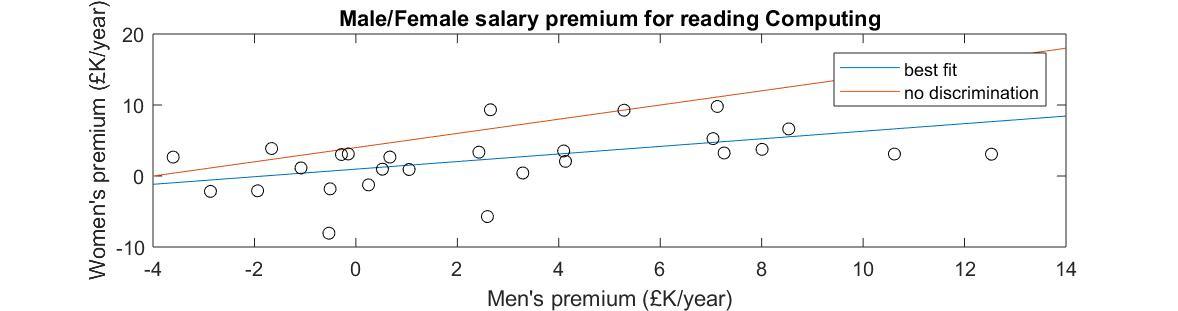
\includegraphics[width=\textwidth]{images/BBCSalaryDatav5.jpg}
\caption{\label{fig:BBC}}
\end{figure*}

\section{UK Higher Education Policy Context}\label{ukhepolicy}

After the UK Government's acceptance of a 2010 review into higher
education funding and student finance~\cite{BIS2010a}, students in
England pay probably the highest\footnote{Or possibly second-highest
after US students, but the US averages in \cite[Table B5.1]{OECD2016a}
conceal an enormous variation.} prices in the world for university
(undergraduate) education: between \pounds6000 and \pounds9000/year
for tuition alone. While this is normally covered by student loans
repaid on an income-contingent basis, essentially through a 9\% income
tax premium, there is evidence that this contributes to lower rates of
planned higher education participation by students from lower social
class groups~\cite{CallenderMason2017a}.

\subsection{Teaching Excellence Framework}

UK universities have been judged, very publicly, on their research for
the last thirty years by a large-scale national Research Assessment
Exercise (RAE), and its successor the Research Evaluation Framework
(REF). This has led to many complaints, largely justified, that
teaching, because it is not measured, is not taken as seriously as
research, certainly in some of the leading research-intensive
universities. Similar comments in the USA can be found in
\cite{Campbelletal2018a}. To counteract this, the Government
introduced a ``Teaching Excellence Framework'' (TEF)\footnote{Now
renamed ``Teaching Excellence and Student Outcomes Framework'', which
is somewhat more descriptive.}, with first grades published in June
2017. The ostensible aim of the TEF was to evaluate the quality of
provision for each higher education provider within the UK. The
initial version of the TEF produced a university-wide assessment on a
three-point (Gold-26\%/Silver-50\%/Bronze-24\%) scale\footnote{For
current scores, see:
\url{https://www.officeforstudents.org.uk/advice-and-guidance/teaching/tef-outcomes/}}. It
in fact used no direct assessment of teaching as such, primarily being
based on historical statistical data, with some concerns raised on the
robustness of the metrics and statistical analysis used to determine
gradings~\cite{gillard:2017}.

In 2018, following an Institutional-level review undertaken in the
previous year, the Office for Students (OfS) conducted a pilot of a
national subject-based TEF. The objective was to provide sufficient
data for prospective students to enable them to undertake an informed
decision about their choice of University and subject of study. This
was particularly pertinent to the UK context as the funding of higher
education has shifted, following several policy
changes~\cite{BIS2010a}, from students receiving means-tested
Government grants to undertaking a loan to pay for their tuition.
% Typical tuition fees are set at around £9k per annum.

%Fifty higher education providers participated in the 2018 pilot, reflecting the diverse range of UK HE within the sector. The pilot collated subjects into 7 groups with 142 subject panel members reviewing the provision. The subject panels consisted of members of the academic community, students, employers and representatives of the professional bodies. Reviewing panels rated a HE provider's subject provision as being either Gold, Silver or Bronze. The Computing subject was grouped with Engineering and Technology. The main goal of the pilot was to inform the development of the subject-TEF methodology to be adopted by the national roll-out currently scheduled for 2019/20. The framework evaluated subject-provision against 6 core metrics. Three of these came directly from the National Student Survey (teaching, academic support and assessment and feedback) one for continuation (retention) and two were related to employment (employment or further study/ highly skilled employment or further study). Reviewers are able to review a provider's metrics against a range of indicators %JHD was "stakeholders"
%including full/part-time students, ethnic diversity, gender, age profile etc. Additionally, supplementary statistics are provided to inform the panel members' review. These include teaching intensity (contact hours in all its various guises) and long-term employment/earnings as measured by the Longitudinal Education Outcomes (LEO) data \cite{DfE2017a}.

The TEF's reliance on employment metrics pre-supposes a strong
correlation between the quality of provision and the employment
prospects/performance of the students. This can be challenging for
some disciplines (e.g. income earning potential is not equally
distributed across all subjects). The intention however is clear. In
the context of students paying their own tuition fees, quality of
provision is being linked to future employment prospects. This
represents an opportunity for UK HE Computing provision. Those
programmes, characteristic of most in computer science, that contain a
placement/internship, are professionally-accredited and whose
curriculum is informed by an employer-led advisory board are
well-placed to do well in the TEF.

\subsection{Degree Apprenticeships}\label{sec:DA}

The UK Government launched ``Degree Apprenticeships'' in
2015~\cite{BIS2015a}, which were described by the then Prime Minister
as ``combining a full degree with the real practical skills gained in
work and the financial security of a regular pay packet''. The
employer pays the tuition cost, but via a national Apprenticeship
Levy~\cite{HMRC2016a}, essentially a 0.5\% payroll tax; large
employers (total payroll over \pounds3m) will find there is no net
cost, while smaller employers can claim 90\% of the cost back from the
government.

Degree Apprenticeships can be either ``Level 6'' (undergraduate/BSc
level) or ``Level 7'' (postgraduate/MSc level''). The Level 6 ones
last three to five years, but typically four\footnote{One such is
detailed at
\url{http://www.aston.ac.uk/study/degree-apprenticeships/employers/degree-apprenticeship-programmes/digital-and-technology-solutions-degree-apprenticeship/}}. The
details of Level 7 apprenticeships have only just been approved at the
time of writing~\cite{IfA2018a}, so it is hard to determine how they will work in
practice. However, the entire Degree Apprenticeship mechanism does
seem to be geared more to large companies capable of supporting a
bespoke programme, as for example is happening in Accountancy, where
the ``Big Four'' firms are enthusiastically supporting such
programmes\footnote{For example:
\url{https://www.pwc.co.uk/careers/school-jobs/jobs/flying-start-degrees.html}}. How
well it can adjust to smaller high-technology companies has yet to be
seen.

\subsection{Sandwich Years}

In the UK context, a university course that includes a period
working in industry (which may also include government, charities, etc) is
generally called a ``sandwich'' course, and in North America the term ``co-op''
is generally used. The most common model in Computing in England,
where the vast majority of students study three-year Bachelor's
degrees, is a year's placement in industry between the second and
final years of study. This is remarkably successful in computing. The
University of Bath has run such courses since its founding (1966),
with about 80\% of students opting to take the sandwich year. There is
statistical evidence for its success wherever it is used in the
UK\footnote{And at least anecdotal evidence elsewhere: ``the co-op
system is a major reason for our [University of Waterloo] success''
\cite{Watt2017a}.}:

\begin{quote} ``{\emph{...those studying sandwich courses enjoy the lowest levels
of unemployment (6\% sandwich vs 15\% non-sandwich), the lowest levels
of non-graduate level employment (6\% sandwich vs 25\% non-sandwich),
and graduates from sandwich courses are twice as likely to be earning
over \pounds20,000 compared to those who did a standard
degree.}}''~\cite{Shadbolt2016a}
\end{quote}

A simplistic remedy would be to require that all students study
sandwich degrees, but this has numerous challenges:

\begin{enumerate}
\item Some students do not wish to, often for valid reasons;
\item The supply of employers willing to offer such placements is
limited, and often they are only offered to a limited number of
universities with whom the employer has built up relations, often
going back decades;
\item The university needs to invest in the process: a successful
sandwich year programme is not a matter of simply allowing students to
intermit their studies.
\end{enumerate}

Hence we should ask ourselves \emph{why} such courses are so
successful (if indeed they are: there is a possible confounding
factor, in that, for those universities with scant support for the
sandwich system, those students that do take a sandwich year will tend
to be the more self-motivated ones, who would probably do well
anyway). There appears to be two classes of reasons: those intrinsic
to the sandwich process, and the skills the sandwich process
confers. The first class is easy to understand: the employer can view
the year as a year-long assessment phase before deciding whether to
offer a permanent job. From the authors' institutional experience,
about 2/3 of sandwich placements result in job offers to the
student. However, it is the second class that we need to investigate
in the hope that non-sandwich courses can learn from them.

%A major one, brought out
%repeatedly by students returning from placement, is team working.

% \subsection{Team/Group working}

% ``Teamwork'' is often identified as a key skill \cite[and many
% others]{ArcherDavidson2008}. Simplistically, then, universities should
% teach it. Indeed, the British Computer Society has long required this
% of degrees it accredits:
% \begin{quote} An ability to work as a member of a development team
% recognising the different roles within a team and different ways of
% organising teams \cite[Requirement 2.3.1]{BCS2018a}.
% \end{quote}
% The problem is that group working is unpopular with students. Most of
% them have never experienced it in their academic work at school, and
% really dislike ``being dragged down'', as they generally put it, by
% others. In many countries, this wouldn't matter, but the UK has (many
% would say ``suffers from'', see, e.g. \cite{Cupples2015a}) the
% National Student Survey \cite{OfS2018a}. The results of this, notably
% the headline ``are you satisfied with your course'' question, are
% pored over intently by university management \cite[Myth
% 3]{OfS2018a}. As well as the quantitative scores, the students submit
% free-text responses, and it does not take many students complaining
% about the group work before the Pro-Vice-Chancellor (Teaching) or
% equivalent\footnote{Whose pay may well be linked to these scores.} is
% beating down the Director of Studies door, saying ``obviously you must
% abolish group work immediately''. The first three authors
% have been Directors of Studies, and can vouch for this.

% However, a BCS-accredited course gives the response ``but our
% accreditation demands it'', whereupon the discussion can evolve into a
% more sensible debate about the size, shape and process of group
% working.
% \par This leads to a curious paradox. Employers value group working
% experience (at a Shadbolt Review focus group, every employer stated
% they always asked potential employees about experience of group
% working), group working experience is only taught because
% accreditation requires it, but employers do not value accreditation.
% ``systems of accreditation more broadly are poorly understood and
% valued by employers, students and HE providers''
% \cite[\P2.12]{Shadbolt2016a}.

% \subsection{Code Review}\label{sec:Code}

% A further aspect of the ``not industry ready'' complaint has recently
% been identified by the Institute of Coding team as part of the
% engagement with industry, and is described by a prominent
% industrialist from the safety-critical sector as follows.
% \begin{quote} We do find we have to train grads how to review stuff
% properly --- both personal (their own stuff) and team/peer
% reviews. While they may have been exposed to the concept of personal
% and peer reviews, none of them have actually been taught how to do it
% properly and how to measure its effectiveness. \cite{Chapman2018c}
% \end{quote} This quote is supported by many Institute of Coding
% industrialists, and also by the work of \cite{Boerstleretal2018a},
% though their conclusion ``Code quality should be discussed more
% thoroughly in educational programs'' is probably too weak. As
% \cite{Chapman2018c} says ``While they may have been exposed to the
% concept of personal and peer reviews'' it is unlikely that many of
% them will actually have practiced it.  One might ask ``but what about
% the group working''?
% \par That is a good question, and one that the Institute of Coding is
% investigating. A provisional answer lies in the nature of group
% working. Practically all BCS-accredited universities meet the
% requirement \cite[Requirement 2.3.1]{BCS2018a} (and ``working with
% others'' \cite[Requirement 2.3.2]{BCS2018a}) by means of a group
% practical project. This is practically always done before the final
% year, both for reasons of balance (BCS also requires an individual
% project amounting to at least 25\% of the final year \cite[Requirement
% 2.5.1]{BCS2018a}) and, more pragmatically, so that the memory of this
% disliked experience will have worn off before the students complete
% the National Student Survey in their final year. Universities with a
% strong sandwich programme also want students to be at least engaged on
% a group project when they go to their interviews.

% But students hate being ``dragged down'' by their fellow team-members
% (it is odd that Directors of Studies and group project lecturers hear
% far less about being ``dragged up''!).  Hence students are very keen
% to have ``their own bit'' of the group activity, and it is difficult
% to have true team responsibility and code reviews.  Various attempts
% are being made at this, e.g. at Bath the use of ``Agile'' methodology
% with testing formally built into the set of sprints, but it is
% probably fair to say that this is an under-researched area.
% \cite{Hundhausenetal2013a} is one of the few pieces of research, but
% they say ``In future research, we would like to systematically
% investigate best practices for building effective
% P[edagogical]C[ode]R[eview] teams''.

% this is the main section? do we have text to rip from the IoC bid
% doc?
% do we want to add note about nomenclature/terminology -- not hugely happy with
% "Institute of Coding'', but this was political, etc...
\section{The Institute of Coding}\label{ioc}

\subsection{Structure}

Formally announced in 2018~\cite{DfE2018a}, but foreshadowed in
2015~\cite{HMG2015a}, the Institute of
Coding\footnote{\url{https://instituteofcoding.org}} is one of the UK
Government's latest responses to the ``digital skills
challenge''~\cite{davenport-et-al:cep2019}. The Institute brings
together a consortium\footnote{For full list of IoC partners, see:
\url{https://instituteofcoding.org/about/team/}} of research- and
teaching-focused universities (primarily based in England due to the
origin of the core funding, along with two Welsh institutions
co-funded through a separate mechanism), large corporates, small- and
medium-sized enterprises (SMEs), established industry groups, experts
in the delivery of distance/non-traditional learning and professional
bodies to develop and deliver innovative, industry-focused education
across the UK. It is explicitly an industry--university collaboration,
with the Government contributing at most 50\% of the project funding.

It brings together for the first time traditional computer science
departments and business schools, leaders in art and design,
innovation in programme delivery, the industry backing of the UK's
leading digital employers, and the leading professional bodies.  The
Institute's vision is that ``every student leaves education with
employment, and that employers and individuals across the UK have
ready access to the skills they need to compete successfully in the
global digital economy''. It is structured around five priority
themes:
%\footnote{\url{https://instituteofcoding.org/about/}}:

\subsection{Theme 1: ``University Learners''}

% This is aimed at understanding, and solving, the ``Skills Mismatch''
% problems (see \S\ref{sec:Skills}). As seen from \S\ref{sec:Code},
% these problems can be quite subtle, and are not addressed by such broad
% requirements as \cite[Requirement 2.3.1]{BCS2018a}.  

{\emph{To increase the number of university learners and improve
employability through innovative learning methods:}}\newline

\noindent This is aimed at understanding, and solving, the various
``Skills Mismatch'' problems to increase the number of university
learners at Levels 6 and 7 (especially in key national priority areas
such as data science and cyber security); as discussed previously,
these problems can be quite subtle, and are not addressed by such
broad requirements as \cite[Requirement 2.3.1]{BCS2018a}. However,
this theme aims to increase graduate employability via stronger
employer links; hence the Institute is also looking at accreditation,
with a view to producing more detailed records, essentially
e-portfolios, of skills achieved, embedding innovative learning
methods into material and delivery across institutions.

% It is possible
% that these may be supported by a open distributed ledger-based
% mechanism, as is being done elsewhere~\cite{RMIT2018a}.

\subsection{Theme 2: ``The Digital Workforce''}

{\emph{To create learning that meets employer needs, enriches the
student experience and provide in-work and flexible learning options
that are viable at scale:}}\newline

\noindent This theme aims to explore alternative delivery models, in
an effort to identify and synthesis best practice -- for both
specialist and generalist provision, as well as educational training
and professional development. There is a strong strand of lifelong
learning: it aims to champion the role of the university as a teaching
and learning partner/provider to equip learners for a career rather
than specific jobs. In practice this is likely to be largely aimed at
degree apprenticeships (see \S\ref{sec:DA}) in the short to medium
term, to draw in more universities to provide Degree Apprenticeships
and other related course models. These are still in their very early
days in computing, and we hope that the Institute will enable best
practice sharing from the beginning. In terms of content, as opposed
to pedagogic practice, this theme is tightly linked with Theme 1,
notably in areas like Cyber security, where there is a great shortage
of non-proprietary teaching material.

\subsection{Theme 3: ``Digitalising the Professions''}

{\emph{To develop learning to address sector-specific digital skills
needs, build an industrial strategy and deliver modular
training:}}\newline

\noindent This theme aims to develop a new industry-facing market of
university-led, industry-valued provision in areas of strategic
importance. The official description ``to transform professions
undergoing digital transformation'' \cite{DfE2018a} is tautologous,
but the consortium aims are to provide a flexible modular digital
masters programme aimed at people in various professions where digital
technologies are changing the job. Especially in sectors where serious
upskilling in necessary (for example, across the creative economy,
automotive, manufacturing, healthcare, the financial sector, etc), and
also to provide various short taster courses in order to widen the
reach of digital skills. As for Theme 2, this will be sharing content
with Theme 1.

\subsection{Theme 4: ``Widening Participation''}

{\emph{To develop a path from first contact to employment, removing
barriers to entry and progress for poorly-served groups:}}\newline

\noindent This is aimed at addressing the systemic issues with
gender and diversity, as identified at the start of this paper:
creating a pipeline, with tailored, inclusive curricula. Since
the Institute bid was submitted and approved, salary
data~\cite{DfE2018d} (see Figure~\ref{fig:BBC}) has been released,
which show the importance of a more nuanced study of the effect of
gender in particular. The UK Government analysis~\cite{DfE2018d}
concentrated on gender, but we are hoping to do similar studies for
computer science with regard to other protected characteristics such
as ethnicity, to better understand and address the barriers, to share
best practice across the sector.

Our current activity is a national survey to better understand the
motivating factors for why different groups of people choose (or not)
to train and work in digital. We are sampling three cohorts: working
people, university learners and 15-18s. The focus is primarily on the
gender difference, and different aspects within the female cohort.

\subsection{Theme 5: ``Knowledge Sharing and Sustainability''}

{\emph{To horizon scan for future digital skills need, disseminate and
share best practice of the project, look at long-term sustainability
and the management of the programme:}}\newline

\noindent This theme is an underpinning theme for the others,
providing longer-term horizon scanning, as well as supporting the
evidence base, policymaking and sustainability through a ``Digital
Skills Observatory''. The Observatory will work with employers and
other stakeholders to identify and anticipate skills gaps through
mapping current needs, to build up an evidence base of research,
analysis and intelligence.  A perverse, but totally natural,
consequence of the REF has been the marginalisation of pedagogy
research in the UK \cite{Cottonetal2018a}. This is particularly acute
in Computing, and can be quantified by noting that Australia, with
less than 40\% of the population of the UK and being over eight times
further away, sends practically the same number of papers to the Koli
Calling conference in Finland as the UK
does~\cite{Simon2016a}. Dissemination of good practice is also low: a
2016 national survey~\cite{murphy-et-al:programming2017} was the first
of its kind in the UK, despite the fact that they had been running for
many years elsewhere~\cite{simon-et-al:sigcse2018}. This has also
prompted a renewed look at how professional body accreditation can
help foster and disseminate good practice~\cite{crick-et-al:cep2020}.

\subsection{Key Challenges}

Delivering as much education as the Institute proposes presumes a
supply of educators; this is a major challenge at all levels for
computing in the UK~\cite{brown-et-al:toce2014}, as it is in many
countries. We have seen a number of challenges in the recruitment and
retention of pre-university teachers (especially in
England~\cite{sentance+waite:2018}), as well as issues with
effectively scaling professional development opportunities at the
national level~\cite{sentance+csizmadia:2017} (for example, subject
knowledge enhancement, pedagogic knowledge, as well and funding to
access courses and higher degree
programmes~\cite{sentance-et-al-wipsce2012,moller+crick:jce2018});
hence one workpackage is devoted to ``educating the educators''.

A further challenge is sustainability. The UK Government funding (for
England) for the Institute is relatively short-term given the systemic
challenges, and indeed will lapse before anyone graduates from a Level
6 (undergraduate/BSc) course or degree apprenticeship. Hence the
Institute needs to build an ecosystem with its academic and industrial
partners to become self-supporting in a very short
timeframe. Furthermore, there are significant challenges to timing and
coordinating devolved funding initiatives across the four nations of
the UK for these types of interventions, especially with potentially
diverging approaches to education and skills policy, including qualifications.

\section{Impact To Date}\label{impact}

Whilst the Institute of Coding is still very much an ongoing ``work in
progress'' -- at the time of writing it is only just two years on from
the official launch announcement, and no-one has yet graduated with an
Institute degree -- there are a number of notable outputs and
achievements, cutting across practice, policy and research, at both
the regional and national level, cutting across all five work
themes. Alongside the various activities and initiatives, it also has
an implicit national cohering role, especially at post-compulsory
level, collaborating with other organisations working on school-level
interventions to create the sustainable ecosystem to address some of
the challenges articulated in this paper.

%mostly Degree Apprenticeships,Masters courses, or joint Masters courses and (Level 7) Degree Apprenticeships.  
There are new degree courses (or new/majorly revised modules on
existing courses) already started in 2018 and 2019, badged as
``Institute of Coding'': see Table~\ref{tab:data}.  It could be argued
that some, particularly the Degree Apprenticeships, might have been
started without the Institute of Coding, but it is certainly the case
that the Institute of Coding has accelerated the process, not least by
short-circuiting\footnote{At the University of Bath, for example, the process of
analysing demand was short-circuited as the IoC was, effectively,
underwriting the start-up costs. Senior management then pushed for
special committee meetings to get the rest of the process completed in
time.} the often labyrinthine ``quality assurance'' processes in
universities, as university leadership, prompted (to say the least) by
the money on offer, had already signed up to the principle. There has
also been a substantial amount of information interchange between IoC
partners over the mechanisms of Degree Apprenticeships, as
universities new to the idea started them: for the majority of IoC
partners, these were the first Degree Apprenticeships the university
had entered into. IoC partners were running four Degree Apprenticeships
in 2018/19 and 16 (so far) in 2019/20.

\begin{table}
  \begin{center}
\caption{IoC Learners as of October 2019\label{tab:data}}
\begin{tabular}{lrr}
  &Courses&Learners\\
    \hline
	BSc. etc. degree courses&5&493\\
	Level 6 Degree Apprenticeships&11&245\\
	Total Level 6 courses&16&738\\
	Modules&19&1258\\
	Total Level 6&35&1996\\\hline
	MSc. etc. degree courses&13&643\\
	Level 7 Degree Apprenticeships&7&153\\
	Total Level 7 courses&20&796\\
	Modules&2&35\\
	Total Level 7&22&831\\\hline
Total Degree courses&18&1136\\
  Total Degree Apprenticeships&18&398\\
                                       \hline
\end{tabular}
\end{center}
\end{table}

In addition, there are a large number of learners on IoC ``taster''
courses. Of the 32,000 learners enrolled (as at the end of September
2019) on IoC courses, over 28,000 are enrolled on these.  The IoC has
completion rate figures for the initial cohorts on the vast majority
of these, and shows a completion rate of 11\%, which, though low,
compares favourably with the MOOC
norm~\cite{ReichRuiperezValiente2019a}. These courses are outside the
usual range of MOOCs in practice, which
\cite{ReichRuiperezValiente2019a} characterises as ``primarily
supporting already-educated learners''.  Further analysis of the IoC
learner profile is on the workplan, to better understand how we can
engage a wider demographic.

From a research and policy perspective, the announce of the Institute
in 2015~\cite{HMG2015a} prompted the baseline research on introductory
programming in UK
universities~\cite{murphy-et-al:programming2017,simon-et-al:sigcse2018},
alongside a significant renewed focus on computer science education in
the UK -- across research, policy and practice -- further reinforced
by the Royal Society's recommendations in its 2017 report on computing
education~\cite{rs:2017}. As we see continued national curriculum and
qualifications reform across the UK, especially in Wales from 2022, as
well as further developments and enhancements of the computing
curriculum in England, we should see more learners progress into
university education with stronger digital skills and more computing
experience; however, this landscape is also complex and fragmented,
with a number of challenges~\cite{roehampton:2018}.

\section{Future Work and Replicability}\label{concl}

We have seen -- and will continue to see -- a number of initiatives,
activities and interventions which may prove useful to other nations
reforming their curricula (both compulsory school-level, as well as
post-compulsory), as well as in the wider aim of developing broader --
sustainable and transferable -- societal digital, data, computational
and engineering skills. There is a long history in the UK and
internationally of university-industry partnerships and
collaborations, especially focusing on R\&D activities e.g. through
the National Centre for Universities and Business (NCUB)\footnote{The
NCUB is an independent and not-for-profit membership organisation that
promotes, develops and supports university-business collaboration
across the UK: \url{http://www.ncub.co.uk}}. This is especially true
for engineering, but these have largely been focused on established
disciplinary boundaries, for example, mechanical, automotive,
aerospace (e.g. Boeing in the UK~\cite{boeinguk:2020}). For
``digital'', this presents a significant widening of scope and sector
coverage, from finance and professional services, through to the
government and the wider public sector, as well as encompassing
traditional IT, software, hardware and telecoms. This also intersects
with more established work on innovation and entrepreneurship (from
both fostering enterprise and entrepreneurship activities with
students, as well as how universities can be more entrepreneurial and
work more closely with industry e.g. Enterprise Educators
UK\footnote{Enterprise Educators UK is the leading independent
membership network for enterprise educators, whose purpose is to
enable excellence in enterprise education:
\url{https://www.enterprise.ac.uk/}}), again with strong European and
international networks. Some of this work has been further reinforced
by impactful work on developing digital skills by Nesta, the UK's innovation
foundation~\cite{nestadeliveringdigitalskills:2018,nestawhatdigitalskills:2018}.

However, we recognise that there has been a significant corpus of
activity in this space, especially internationally, linking to wider
initiatives to promote and support computer science education
e.g. Computer Science Education Week
(CSEdWeek)\footnote{\url{https://csedweek.org}} and
CSforAll\footnote{\url{https://www.csforall.org}}. Across the UK, the
high-profile and impactful work of organisations such as Computing At
School (CAS), Raspberry Pi Foundation, Code Club, Technocamps, {\it et
al\/}., has led to a \pounds84m investment in 2018 for a National
Centre for Computing Education\footnote{See:
\url{https://teachcomputing.org/}} in England. This has also been
supported by a wide range of activities (including accreditation,
curriculum and qualifications development) by key professional
bodies/learned societies, such as BCS, The Chartered Institute for IT
and the Institution of Engineering and Technology (IET).

More specifically related to the aims and activities of the Institute
of Coding, we have seen a multitude of initiatives purporting to
quickly address the digital skills gap; it is thus important to
evaluate what has been successful, and perhaps more importantly, not
to replicate past failures. For example: high-profile ``coding
universities'' (for example, CODE in Berlin\footnote{CODE is a private
university of applied sciences that is embedded into the vibrant
network of Berlin’s digital economy: \url{https://code.berlin/en/}};
microdegrees and MOOCs (e.g. Elements of AI, a series of free online
courses created by the University of
Helsinki\footnote{\url{https://www.elementsofai.com}}; industry boot
camps and brokering/matching developers with the top companies
(e.g. HackerRank, which is increasingly popular in UK
universities\footnote{\url{https://www.hackerrank.com}}); public
sector/civic service collaborations (e.g. Code for
America\footnote{Code for America uses the principles and practices of
the digital age to ``{\emph{improve how government serves the American
public, and how the public improves government}}'':
\url{https://www.codeforamerica.org}}; to baselining and
identification of best practice (e.g. in programming and software
engineering~\cite{murphy-et-al:programming2017}), cybersecurity
education (e.g.~\cite{crick-et-al:fie2019, itnowcyber:2019}) and
degree accreditation~\cite{crick-et-al:cep2020}.

When establishing a model for viewing computer science education
initiatives, it is apparent that there is substantial diversity
between education systems -- from formal school curricula through to
tertiary education, as well as wider education policy and funding --
and this can create obstacles when trying to understand progress made
in one country and potentially replicate it in
another~\cite{hubwieser:2013,falkner-et-al:2019}. This is particularly
relevant to the devolved (and diverging) educational systems of the
UK, as well as the variety of its disparate interventions, especially
formal curricula and post-compulsory/tertiary education.  There remain
significant challenges, particularly around connectedness and
coherency of policy, as well as bridging the gap between the
expectations and evolving requirements of (higher) education and
industry. However, two overarching themes are apparent:

\begin{itemize}
\item Firstly, such effort has to be viewed as a coordinated
multi-pronged approach, requiring an overarching holistic strategy,
co-designing/co-constructing/co-producing with universities, colleges,
employers including but not limited to key digital industry partners,
local and national government, as well as young people, parents and
the wider public; it must also cohere with other related education and
skills interventions, especially in national curricula and compulsory
education pathways;

\item Secondly, there is a need to overcome the challenges of
recurrent funding and support to ensure long-term sustainability of
the interventions, as well as parity of opportunity for all
young learners. In essence, it must be viewed as a long-term,
strategic activity, as part of core funding, aligning to related
national policy priorities (especially economic policy, such as the UK
Industrial Strategy~\cite{ukis:2017}). Whilst we do not necessarily
recommend replicating some of the policy or governance structures
under which the UK operates (especially national quality assessment
exercises such as the TEF), we have seen how they can provide a useful
policy lever for initiatives such as the Institute.
\end{itemize}

The Institute of Coding thus aims in the longer term to fulfil an
implicit national cohering role, collaborating with other
organisations working on cognate interventions; in particular:
providing a platform for conducting research activities; building the
evidence base and informing policy; supporting degree/qualifications
accreditation and standards alongside key professional bodies; as well
as changing the wider perception -- and economic, societal and
cultural importance -- of `ICT', `digital', `coding' and other cognate
skills. Whilst it is clear these goals will not be fully completed in
a 3-5 year timescale, the Institute of Coding will provide a strong
foundation for continued work in this area.

\section*{Acknowledgements}

({\emph{Removed for double-blind reviewing}})

% This work was supported by the Institute of Coding (IoC), which received
% \pounds20m of funding from the Office for Students (OfS), as well as
% support from the Higher Education Funding Council for Wales (HEFCW).

% We are grateful to the IoC Observatory staff, especially Dr Fiona
% MacGill (University of Bath), for the data collection. The first
% author is also grateful to Dr Matt Dickson (University of Bath) for
% discussions about undergraduate degrees and labour market returns in
% the UK~\cite{DfE2018d}, but any mistakes are the authors' alone.

% trigger a \newpage just before the given reference
% number - used to balance the columns on the last page
% adjust value as needed - may need to be readjusted if
% the document is modified later
\IEEEtriggeratref{47}
% The "triggered" command can be changed if desired:
%\IEEEtriggercmd{\enlargethispage{-5in}}

\bibliographystyle{IEEEtran}      % basic style, author-year citations
\bibliography{EDUCON2020} 

\end{document}
